\documentclass[letterpaper]{report}
%\usepackage[utf8]{inputenc}
\usepackage[T1]{fontenc}
\usepackage{RJournal}
\usepackage{amsmath,amssymb,array}
\usepackage{booktabs}

%% load any required packages here

\usepackage[spanish]{babel}
\usepackage{graphicx}

\hypersetup{pdftitle={rvad: perfiles verticales de viento a patir de datos de radares
meteorológicos},
            pdfkeywords={Meteorología; Radar; Viento}}


\hypersetup{pdfauthor={Paola Corrales, Elio Campitelli}}


%\usepackage[hidelinks]{hyperref}

\urlstyle{same}  % don't use monospace font for urls
\usepackage{color}
\usepackage{fancyvrb}
\newcommand{\VerbBar}{|}
\newcommand{\VERB}{\Verb[commandchars=\\\{\}]}
\DefineVerbatimEnvironment{Highlighting}{Verbatim}{commandchars=\\\{\}} 
% Add ',fontsize=\small' for more characters per line
\usepackage{framed}
\definecolor{shadecolor}{RGB}{248,248,248}
\newenvironment{Shaded}{\begin{snugshade}}{\end{snugshade}}
\newcommand{\AlertTok}[1]{\textcolor[rgb]{0.94,0.16,0.16}{#1}}
\newcommand{\AnnotationTok}[1]{\textcolor[rgb]{0.56,0.35,0.01}{\textbf{\textit{#1}}}}
\newcommand{\AttributeTok}[1]{\textcolor[rgb]{0.77,0.63,0.00}{#1}}
\newcommand{\BaseNTok}[1]{\textcolor[rgb]{0.00,0.00,0.81}{#1}}
\newcommand{\BuiltInTok}[1]{#1}
\newcommand{\CharTok}[1]{\textcolor[rgb]{0.31,0.60,0.02}{#1}}
\newcommand{\CommentTok}[1]{\textcolor[rgb]{0.56,0.35,0.01}{\textit{#1}}}
\newcommand{\CommentVarTok}[1]{\textcolor[rgb]{0.56,0.35,0.01}{\textbf{\textit{#1}}}}
\newcommand{\ConstantTok}[1]{\textcolor[rgb]{0.00,0.00,0.00}{#1}}
\newcommand{\ControlFlowTok}[1]{\textcolor[rgb]{0.13,0.29,0.53}{\textbf{#1}}}
\newcommand{\DataTypeTok}[1]{\textcolor[rgb]{0.13,0.29,0.53}{#1}}
\newcommand{\DecValTok}[1]{\textcolor[rgb]{0.00,0.00,0.81}{#1}}
\newcommand{\DocumentationTok}[1]{\textcolor[rgb]{0.56,0.35,0.01}{\textbf{\textit{#1}}}}
\newcommand{\ErrorTok}[1]{\textcolor[rgb]{0.64,0.00,0.00}{\textbf{#1}}}
\newcommand{\ExtensionTok}[1]{#1}
\newcommand{\FloatTok}[1]{\textcolor[rgb]{0.00,0.00,0.81}{#1}}
\newcommand{\FunctionTok}[1]{\textcolor[rgb]{0.00,0.00,0.00}{#1}}
\newcommand{\ImportTok}[1]{#1}
\newcommand{\InformationTok}[1]{\textcolor[rgb]{0.56,0.35,0.01}{\textbf{\textit{#1}}}}
\newcommand{\KeywordTok}[1]{\textcolor[rgb]{0.13,0.29,0.53}{\textbf{#1}}}
\newcommand{\NormalTok}[1]{#1}
\newcommand{\OperatorTok}[1]{\textcolor[rgb]{0.81,0.36,0.00}{\textbf{#1}}}
\newcommand{\OtherTok}[1]{\textcolor[rgb]{0.56,0.35,0.01}{#1}}
\newcommand{\PreprocessorTok}[1]{\textcolor[rgb]{0.56,0.35,0.01}{\textit{#1}}}
\newcommand{\RegionMarkerTok}[1]{#1}
\newcommand{\SpecialCharTok}[1]{\textcolor[rgb]{0.00,0.00,0.00}{#1}}
\newcommand{\SpecialStringTok}[1]{\textcolor[rgb]{0.31,0.60,0.02}{#1}}
\newcommand{\StringTok}[1]{\textcolor[rgb]{0.31,0.60,0.02}{#1}}
\newcommand{\VariableTok}[1]{\textcolor[rgb]{0.00,0.00,0.00}{#1}}
\newcommand{\VerbatimStringTok}[1]{\textcolor[rgb]{0.31,0.60,0.02}{#1}}
\newcommand{\WarningTok}[1]{\textcolor[rgb]{0.56,0.35,0.01}{\textbf{\textit{#1}}}}

\providecommand{\keywords}[1]{\noindent\textbf{Palabras clave:} #1}
\providecommand{\tightlist}{%
\setlength{\itemsep}{0pt}\setlength{\parskip}{0pt}}

\usepackage{subfig} 


\begin{document}

%% do not edit, for illustration only
\sectionhead{rvad: perfiles verticales de viento a patir de datos de radares
meteorológicos}
\year{2019}

\begin{article}

\title{rvad: perfiles verticales de viento a patir de datos de radares
meteorológicos}

\author{
Paola Corrales , 
Elio Campitelli }

\maketitle


\keywords{ Meteorología  -  Radar  -  Viento }

\hypertarget{introduccion}{%
\section{Introducción}\label{introduccion}}

El estudio y monitoreo del viento en niveles bajos de la atmósfera es de
suma importancia ya que el mismo afecta diversos procesos que tienen un
alto impacto en la sociedad. Por ejemplo influye en el desarrollo y
severidad de las tormentas de manera directa por la rotación del viento
con la altura en los primeros kilómetros. También afectan de manera
indirecta a través de procesos de mayor escala, como el transporte de
humedad desde el Amazonas hacia el sur de Sudamerica. Sin embargo, las
mediciones de viento en superficie tienen una resolución espacial y
temporal muy baja y normalmente se realizan únicamente a 10 metros de
altura.

Los radares Doppler pueden medir el viento en un volumen de aire cada 5
o 10 minutos. Por esto tienen una gran potencialidad para estimar la
variación del viento con la altura. Pero las variables medidas por el
radar requieren algoritmos de procesamiento y técnicas de control de
calidad de datos. Implementarlos en R permite extender el uso del
lenguaje a otras diciplinas como la meteorología, tanto en investigación
como en tareas operativas de monitoreo del tiempo.

En este trabajo se presenta el paquete
\href{https://github.com/paocorrales/rvad}{rvad} que implementa de la
técnica \emph{Velocity Azimuth Display} (VAD) para estimar un perfil
vertical de las componentes horizonaltes del viento a partir del viento
medido por el radar.

\hypertarget{algoritmo}{%
\section{Algoritmo}\label{algoritmo}}

Un radar gira sobre su eje enviando pulsos de energía electromagnética
en cada ángulo horizontal o \emph{azimut}. Al terminar cada giro de 360
grados, cambia su \emph{ángulo de elevación} y repite el proceso. El
pulso de radar recorre una determinada distancia (\emph{rango}) y en el
camino puede ser interceptado por gotas de agua, granizo o, en casos sin
nubosidad, insectos.

Una de las variables medidas por el radar es la velocidad radial o
Doppler, que corresponde a la componente radial del viento, es decir, la
proyección del viento en la dirección de la propagación del haz de
radar. Valores negativos corresponden a movimientos hacia el radar y
valores positivos a movimientos desde el radar, mientras que el valor
nulo ocurre en las regiones donde el viento es perpendicular a la
trayectoria del haz.

La técnica VAD aprovecha el comportamiento sinusoidal del viento radial
para cada rango y ángulo de elevación y ajusta estos datos a una función
de la forma \(v \cos(\theta) \cos(\phi) + u \cos(theta) sin(\phi)\)
donde \(\theta\) es el ángulo de elevación y \(\phi\) el azimuth.
Estimando la propagación del haz del radar, es posible obtener una
altura vertical para los valores del viento zonal (\(u\)) y meridional
(\(v\)). Finalmente, bajo ciertas condiciones es posible realizar un
promedio de todas las estimaciones de \(u\) y \(v\) para obtener un
perfil vertical de viento representativo del volumen de atmósfera
escaneado por el radar.

\hypertarget{implementacion}{%
\section{Implementación}\label{implementacion}}

El paquete \texttt{rvad} implementa el algoritmo VAD presentado por
Browning and Wexler (1968) e incluye una serie de controles de calidad
que buscan solucionar problemas típicos asociados a los datos de radar.

En primer lugar, la función \texttt{vad\_fit()} toma vectores con la
velocidad radial, el azimuth, el rango y el ángulo de elevación y
realiza un ajuste sinusoidal para cada anillo de datos (las
observaciones para un rango y ángulo de elevación particular). Además
realiza los siguientes controles de calidad:

\textbf{Antes del ajuste:}

\begin{itemize}
\tightlist
\item
  Cuenta la cantidad de datos faltantes en el anillo y si supera un
  umbral máximo \texttt{max\_na} el anillo es rechazado.
\item
  Busca gaps o huecos continuos de datos faltantes y rechaza aquellos
  anillos con huecos mayores al umbral \texttt{max\_consecutive\_na}.
\end{itemize}

\textbf{Luego del ajuste:}

\begin{itemize}
\tightlist
\item
  El algoritmo rechaza los anillos cuyo ajuste tiene un \(R^2\) menor al
  umbral \texttt{r2\_min}.
\end{itemize}

El data frame resultante puede ser visualizando fácilmente con el método
\texttt{plot()}.

\begin{Shaded}
\begin{Highlighting}[]
\KeywordTok{library}\NormalTok{(rvad)}
\KeywordTok{library}\NormalTok{(ggplot2)}
\NormalTok{VAD <-}\StringTok{ }\KeywordTok{with}\NormalTok{(radial_wind, }\KeywordTok{vad_fit}\NormalTok{(radial_wind, azimuth, range, elevation))}
\KeywordTok{plot}\NormalTok{(VAD) }\OperatorTok{+}\StringTok{ }
\StringTok{  }\KeywordTok{scale_color_discrete}\NormalTok{(}\DataTypeTok{guide =} \StringTok{"none"}\NormalTok{) }\OperatorTok{+}
\StringTok{  }\KeywordTok{labs}\NormalTok{(}\DataTypeTok{x =} \StringTok{"Magnitud del viento (m/s)"}\NormalTok{, }\DataTypeTok{y =} \StringTok{"Altura (m)"}\NormalTok{)}
\NormalTok{wind_profile <-}\StringTok{ }\KeywordTok{vad_regrid}\NormalTok{(VAD, }\DataTypeTok{layer_width =} \DecValTok{100}\NormalTok{)}
\KeywordTok{plot}\NormalTok{(wind_profile) }\OperatorTok{+}
\StringTok{  }\KeywordTok{labs}\NormalTok{(}\DataTypeTok{y =} \StringTok{"Magnitud del viento (m/s)"}\NormalTok{, }\DataTypeTok{x =} \StringTok{"Altura (m)"}\NormalTok{)}
\end{Highlighting}
\end{Shaded}

\begin{figure}

{\centering \subfloat[\label{fig:vad_fit1}]{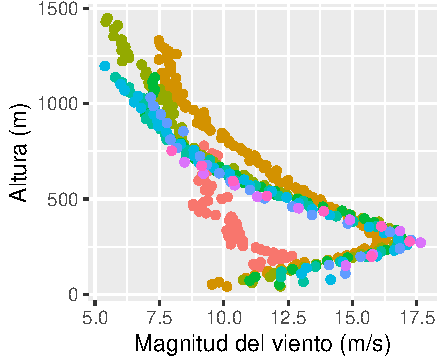
\includegraphics{Resumen_files/figure-latex/vad_fit-1} }\subfloat[\label{fig:vad_fit2}]{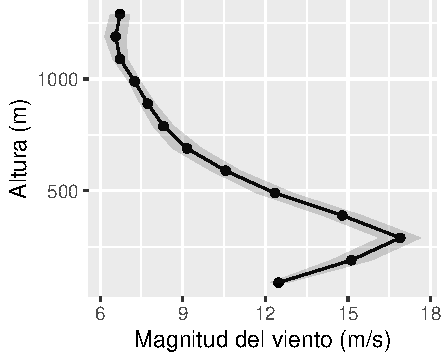
\includegraphics{Resumen_files/figure-latex/vad_fit-2} }

}

\caption{Estimación del viento obtenido a partir de (a) vad\_fit() y (b) vad\_regrid()}\label{fig:vad_fit}
\end{figure}

En segundo lugar la función \texttt{vad\_regrid()} toma el data frame
generado por \texttt{vad\_fit()} y genera un único perfil vertical en
una grilla regular utilizando un regresión local de orden 1. La función
devuelve el valor de \(u\) y \(v\) para cada nivel de altura y el
intervalo de confianza asociado.

Estas dos funciones principales deben ser utilizadas en serie para
obtener el pertfil vertical. El paquete las implementa por separado dado
que es importante analizar el ajuste individual de cada anillo en
función del ángulo de elevación para evaluar la calidad de los datos y
ajustar los controles de calidad.

\hypertarget{referencias}{%
\section*{Referencias}\label{referencias}}
\addcontentsline{toc}{section}{Referencias}

\hypertarget{refs}{}
\leavevmode\hypertarget{ref-Browning1968}{}%
Browning, K. A., and R. Wexler. 1968. ``The Determination of Kinematic
Properties of a Wind Field Using Doppler Radar.'' \emph{Journal of
Applied Meteorology} 7 (1): 105--13.
\href{https://doi.org/10.1175/1520-0450(1968)007\%3C0105:TDOKPO\%3E2.0.CO;2}{https://doi.org/10.1175/1520-0450(1968)007\textless0105:TDOKPO\textgreater2.0.CO;2}.



\address{Paola Corrales\\
Centro de Investigaciones del Mar y la Atmósfera UBA-CONICET\\
\email{paola.corrales@cima.fcen.uba.ar}}

\address{Elio Campitelli\\
Centro de Investigaciones del Mar y la Atmósfera UBA-CONICET\\
}




\end{article}
\end{document}

